\scanpage{41}
\diagram{\begin{tikzcd}[ampersand replacement=\&]X\arrow[d]\\S\end{tikzcd}}
\figure{\begin{tikzpicture}
\node[inner sep=5pt] (h) {$\underline{\mathcal H}^{1}(X/S;\underline{\operatorname{Hom}}_{S-gr}(\unsure{\gamma|\sigma},G))\xrightarrow{\sim}\underline{\operatorname{Hom}}_{S-gr}(\gamma,\underline{\mathcal H}^{1}(X/S,G))$};
\draw (h.north west)--(h.north east);\draw (h.south west)--(h.south east);\draw ([yshift=-2pt]h.north west)--([yshift=2pt]h.south west);
\end{tikzpicture}}
isom de foncteurs, \deleted{pour} quand tout est \uline{affine} sur $S$ (?)
\[
\boxed{\underline{\mathcal H}^{1}(X/S;\underline{\operatorname{Ext}}^{1}_{S-gr}(\gamma,G))
\simeq\underline{\operatorname{Ext}}^{1}_{S-gr}(\gamma,\mathcal H^{1}(X/S,G))}
\]
Sous quelles conditions ???

\[\unsure{P_X|\rho_X}\]
\diagram{\begin{tikzcd}[ampersand replacement=\&, column sep=large]
X\arrow[d,no head]\&\deleted{\unsure{\gamma_X}}\&\deleted{\unsure{\gamma_X\times\gamma_X}}\\
S\&\gamma\&\gamma\times\gamma
\end{tikzcd}}
\[
\mathcal H^1(X/S,\underline{\operatorname{Hom}}_{S-gr}(\gamma,G))\longrightarrow
\operatorname{Hom}(\gamma,\mathcal H^1(X/S,G))
\]
\[
\mathcal H^1(X,\operatorname{Hom}(A;B))\simeq
\]
\margin{$\deleted{\unsure{\operatorname{Ext}_{X/S}|\operatorname{Ext}(X,B)}}$}
\figure{\begin{tikzpicture}
\node[inner sep=5pt] (d) {\diagram{\begin{tikzcd}[ampersand replacement=\&, row sep=large]
H^1(X/S;\underline{\operatorname{Hom}}_{S-gr}(\gamma,G))\arrow[d,shift right=18mm]\\
\underline{\operatorname{Hom}}_{S-gr}(\gamma,H^1(X/S,G))
\end{tikzcd}}};
\draw (d.north west)--([xshift=8mm]d.north east);\draw (d.south west)--([xshift=8mm]d.south east);\draw (d.north west)--(d.south west);\draw (d.north east)--(d.south east);
\end{tikzpicture}}
\margin{40}
